\documentclass[11pt,]{article}
\usepackage[left=1in,top=1in,right=1in,bottom=1in]{geometry}
\newcommand*{\authorfont}{\fontfamily{phv}\selectfont}
\usepackage[]{mathpazo}


  \usepackage[T1]{fontenc}
  \usepackage[utf8]{inputenc}



\usepackage{abstract}
\renewcommand{\abstractname}{}    % clear the title
\renewcommand{\absnamepos}{empty} % originally center

\renewenvironment{abstract}
 {{%
    \setlength{\leftmargin}{0mm}
    \setlength{\rightmargin}{\leftmargin}%
  }%
  \relax}
 {\endlist}

\makeatletter
\def\@maketitle{%
  \newpage
%  \null
%  \vskip 2em%
%  \begin{center}%
  \let \footnote \thanks
    {\fontsize{18}{20}\selectfont\raggedright  \setlength{\parindent}{0pt} \@title \par}%
}
%\fi
\makeatother




\setcounter{secnumdepth}{3}

\usepackage{longtable,booktabs}

\usepackage{graphicx,grffile}
\makeatletter
\def\maxwidth{\ifdim\Gin@nat@width>\linewidth\linewidth\else\Gin@nat@width\fi}
\def\maxheight{\ifdim\Gin@nat@height>\textheight\textheight\else\Gin@nat@height\fi}
\makeatother
% Scale images if necessary, so that they will not overflow the page
% margins by default, and it is still possible to overwrite the defaults
% using explicit options in \includegraphics[width, height, ...]{}
\setkeys{Gin}{width=\maxwidth,height=\maxheight,keepaspectratio}

\title{``Asociación y abundancia relativa de especies de la familia Rubiaceae
en la parcela permanente Isla Barro Colorado''\\
Subtítulo\\
Subtítulo  }



\author{\Large J. Alberto Meléndez Juan\vspace{0.05in} \newline\normalsize\emph{Universidad Autónoma de Santo Domingo (UASD)}  }


\date{}

\usepackage{titlesec}

\titleformat*{\section}{\normalsize\bfseries}
\titleformat*{\subsection}{\normalsize\itshape}
\titleformat*{\subsubsection}{\normalsize\itshape}
\titleformat*{\paragraph}{\normalsize\itshape}
\titleformat*{\subparagraph}{\normalsize\itshape}

\titlespacing{\section}
{0pt}{36pt}{0pt}
\titlespacing{\subsection}
{0pt}{36pt}{0pt}
\titlespacing{\subsubsection}
{0pt}{36pt}{0pt}





\newtheorem{hypothesis}{Hypothesis}
\usepackage{setspace}

\makeatletter
\@ifpackageloaded{hyperref}{}{%
\ifxetex
  \PassOptionsToPackage{hyphens}{url}\usepackage[setpagesize=false, % page size defined by xetex
              unicode=false, % unicode breaks when used with xetex
              xetex]{hyperref}
\else
  \PassOptionsToPackage{hyphens}{url}\usepackage[unicode=true]{hyperref}
\fi
}

\@ifpackageloaded{color}{
    \PassOptionsToPackage{usenames,dvipsnames}{color}
}{%
    \usepackage[usenames,dvipsnames]{color}
}
\makeatother
\hypersetup{breaklinks=true,
            bookmarks=true,
            pdfauthor={J. Alberto Meléndez Juan (Universidad Autónoma de Santo Domingo (UASD))},
             pdfkeywords = {palabra clave 1, palabra clave 2},  
            pdftitle={``Asociación y abundancia relativa de especies de la familia Rubiaceae
en la parcela permanente Isla Barro Colorado''\\
Subtítulo\\
Subtítulo},
            colorlinks=true,
            citecolor=blue,
            urlcolor=blue,
            linkcolor=magenta,
            pdfborder={0 0 0}}
\urlstyle{same}  % don't use monospace font for urls

% set default figure placement to htbp
\makeatletter
\def\fps@figure{htbp}
\makeatother

\usepackage{amsmath}

\usepackage{pdflscape} \newcommand{\blandscape}{\begin{landscape}} \newcommand{\elandscape}{\end{landscape}}


% add tightlist ----------
\providecommand{\tightlist}{%
\setlength{\itemsep}{0pt}\setlength{\parskip}{0pt}}

\begin{document}
	
% \pagenumbering{arabic}% resets `page` counter to 1 
%
% \maketitle

{% \usefont{T1}{pnc}{m}{n}
\setlength{\parindent}{0pt}
\thispagestyle{plain}
{\fontsize{18}{20}\selectfont\raggedright 
\maketitle  % title \par  

}

{
   \vskip 13.5pt\relax \normalsize\fontsize{11}{12} 
\textbf{\authorfont J. Alberto Meléndez Juan} \hskip 15pt \emph{\small Universidad Autónoma de Santo Domingo (UASD)}   

}

}








\begin{abstract}

    \hbox{\vrule height .2pt width 39.14pc}

    \vskip 8.5pt % \small 

\noindent Resumen del manuscrito


\vskip 8.5pt \noindent \emph{Keywords}: palabra clave 1, palabra clave 2 \par

    \hbox{\vrule height .2pt width 39.14pc}



\end{abstract}


\vskip 6.5pt


\noindent  \section{Introducción}\label{introducciuxf3n}

Las comunidades vegetales de los bosques neotropicales ejemplifican la
diversidad y complejidad ecológica de la región tropical. El estudio
continuo de su riqueza y abundancia relativa permite identificar las
especies raras, las cuales son más vulnerables a los cambios en su
hábitat y por lo tanto propensas a extinguirse localmente (Volkov,
Banavar, Hubbell, \& Maritan, 2003). Claramente existe entonces la
necesidad de conocer como se encuentran asociadas estas especies entre
sí dentro de las comunidades ecológicas para ayudar a comprender los
factores que inciden en su conservación (Moreno, 2001).

La familia Rubiaceae es un importante grupo de plantas vasculares de
distribución cosmopolita con una marcada diversidad en regiones
tropicales y subtropicales (Davis et al., 2009). Muchas de las especies
que componen esta familia se encuentran adaptadas a la vida en la
penúmbra, y prosperan bajo la sombra del dosel selvatico. En estas
selvas tropicales, el grado de ordenación y riqueza de las comunidades
que componen el sotobosque dependen en gran medida de interacciónes
entre las distintas especies (Torres-Leite et al., 2019), además de
factores ambientales de su hábitat, ya que muchas de estas especies
estan adaptadas a rangos elevados de ácidez y otras condiciones
específicas de los componentes del suelo, como la concentración de
distintos metales (Jansen, Robbrecht, Beeckman, \& Smets, 2000). Es
preciso señalar que trabajos anteriores (Condit et al., 2002) sobre el
bosque tropical panameño y el grado de reemplazo entre especies de
distintas comunidades o diversidad beta, sugieren que la disimilaridad
tiende a aumentar en función de la distancia a la cual se encuentran
separadas en el espacio. Sin embargo, estos trabajos no restan
importancia a la variabilidad del hábitat y se toman en cuenta en este
estudio, ya que un acercamiento inicial a los datos de abundancia de las
distintas especies de Rubiaceae en Barro Colorado arrojó indicios de
posibles patrones acerca de su distribución, y se plantea la posibilidad
de que existan especies con algún grado de asociación respecto a las
variables ambientales que allí imperan. Actualmente, la distribución de
la abundancia de las especies puede explicarse por medio de distintos
mecanismos los cuales definen una comunidad en particular. Pudiendo
existir en esta una proporción variable de especies dominantes, con una
abundancia alta en comparación con las especies raras y menos
abundantes, las medidas para la distribución de la abundancia relativa
se encuentran sujetas a interacciones que aún no se conocen del todo ni
en qué grado inciden en la estructura de la comunidad (Néda, Horvat,
Toháti, Derzsi, \& Balogh, 2008). El presente estudio intenta la
relación entre abundancia relativa de especies de la familia Rubiaceae y
su distribución en una porción de bosque tropical en la parcela
permanente Barro Colorado Island (en lo adelante BCI), Colón, Panamá.
Las parcelas permanentes como BCI son una excelente fuente de datos
demográficos y posibilitan el estudio continuo de la diversidad a nivel
local y contribuyen a medir el aporte de la familia Rubiaceae a la
diversidad de su comunidad. En ese sentido, este trabajo aprovecha la
información disponible (Hubbell, Condit, \& Foster, 2021) y herramientas
de libre acceso (Martínez Batlle, 2020) para conocer posibles patrones
de asociación entre estas especies, y como varía la diversidad con
respecto a las características del hábitat en el cual crecen estas
poblaciones de plantas y otras condiciones ambientales mediante análisis
estadístico de datos de los censos realizados en Barro Colorado.

\section{Metodología}\label{metodologuxeda}

La parcela permanente BCI es una estación de censo permanente
administrada por el Center for Tropical Forest Science ubicada en el
centro de la isla artificial Barro Colorado, con las coordenadas
09\(^\circ\)~09'N, 079\(^\circ\)~50'O. La parcela consiste en un
polígono de 50 hectáreas cuadradas en el cual se han contabilizado todos
los arboles con más de 10 mm de diámetro a la altura del pecho cada
cinco años desde 1985 (Hubbell \& Foster, 1983, Hubbell et al. (1990),
Condit, Chisholm, \& Hubbell (2012), Condit, Pérez, Lao, Aguilar, \&
Hubbell (2017)); en este estudio se utilizaron las datos del censo
realizado en 2015.

Los datos referentes a estos censos fueron manejados en R (R Core Team
(2020)) partiendo de su disposición en dos matrices de comunidad y
ambiental de cada uno de los 50 cuadrantes de una hectárea que componen
BCI (Martínez Batlle, 2020). Estas matrices contienen datos de las
variables ambientales como condiciones edáficas, tipo de hábitat,
variación topográfica y clasificación etaria del bosque, y datos
demográficos y georeferenciación espacial de todos los individuos
censados. Se adaptaron \emph{scripts} reproducibles recuperados de
Martínez Batlle (2020), utilizando la colección de paquetes
multifuncionales \emph{Tidyverse} (Wickham, 2017), paquetes gráficos y
de procesamiento de datos espaciales para la representación de mapas y
figuras como \texttt{mapview} (Appelhans, Detsch, Reudenbach, \&
Woellauer, 2019) y \emph{simplefeatures} (Pebesma, 2018); y herramientas
de análisis estadístico como \texttt{vegan} (Oksanen et al., 2019),
\texttt{indicspecies} (De Caceres \& Legendre, 2009), entre otros (ver
\ref{información suplementaria}).

A fin de conocer las características distintivas de los datos
conservados en las matrices de comunidad y ambiental, se realizó un
análisis exploratorio de los mismos que incluyó la visualización de
gráficos, tablas, mapas de los cuadrantes de una hectárea y paneles de
correlación lineal entre variables de ambas matrices, esto permitió
obtener una perspectiva general y ayudó a determinar los procedimientos
posteriores que se detallan acontinuación.

\section{Medición de asociación}\label{mediciuxf3n-de-asociaciuxf3n}

Para las pruebas de medición de asociación, se calculó la distancia
Euclidea entre los cuadrantes considerados como objetos. Para esto, fué
requerida la transformada de la matríz de comunidad por el método de
Hellinger, el cual consiste en la radicación al cuadrado de la
abundancia relativa \(y_{ij}\) (cociente resultante de cada valor de
abundancia entre la suma de los sitios) como muestra la fórmula
\ref{eq:hell_transf}. Donde \emph{j} refiere a cada especie o columna en
la matríz, \emph{i} es la fila o cuadrante e \emph{i+} representa la
suma de filas de la matríz de la i-ésima fila (Legendre \& Gallagher,
2001). Además, la distancia euclidea entre cuadrantes en cuanto a la
ocurrencia de especies fué evaluada aplicando el índice de disimilaridad
de Jaccard de la matríz normalizada, con valores de abundancia
convertidos en valores binarios (Borcard, Gillet, \& Legendre, 2018). De
la misma manera, se utiliza la métrica de Jaccard aplicada a la matriz
de comunidad transpuesta y convertida a datos de presencia/ausencia para
medir el grado de asociación entre especies.

\begin{equation} \label{eq:hell_transf}
y' = \sqrt{\frac{y_{ij}}{y_{i+}}}
\end{equation}

Para poder comparar la relación entre las especies según su abundancia
númerica, se utilizó estandarización chi-cuadrado de la matríz de
comunidad transpuesta (Legendre \& Gallagher, 2001). La ocurrencia entre
las especies y su distribución en BCI fué examinada por medio de el
coeficiente de correlación entre rangos de Spearman para medir el grado
de asosiación entre las variables riqueza númerica de especies y la
abundancia con las variables ambientales geomorfológicas y la
composición química del suelo(Borcard et al., 2018).

\section{Análisis de agrupamiento}\label{anuxe1lisis-de-agrupamiento}

Tanto el método jerarquico aglomerativo de asociación entre pares de
cuadrantes (según su composición de especies) bajo el criterio de enlace
completo y el método Ward basado en la varianza mínima fueron utilizados
en el análisis de agrupamiento para contrastar su eficacia y lograr
conseguir grupos consistentes entre ambos (Borcard et al., 2018). Estos
generaron dendrogramas que posteriormente fueron examinados en paralelo
con la matríz de distancias de cuerdas (Legendre \& Gallagher, 2001)
utilizando correlación cofenética entre ambas para determinar el número
ideal de grupos conformados por los cuadrantes. Se hizo uso de los
métodos de remuestreo bootstrap y boostrap multiescalar para conocer la
probabilidad de exito en la inferencia del número de grupos y la
identidad de sus componentes (Borcard et al., 2018). Las reparticiones
se basaron en una probabilidad de 91\% o más de acierto para el metodo
bootstrap y de un 95\% para boostrap multiescalar. Estos resultados
sugieren 2 grupos con 95\% o más de confianza en cada caso para el
metodo Ward; 12 grupos sugeridos por los estandares establecidos para
bootstrap y 10 grupos para bootstrap multiescalar para el metodo por
medio de enlace completo. Para cada método de agrupamiento se
consideraron como válidos: un grupo con 34 cuadrantes y un segundo
conformado por 16 formulados por el método Ward, y dos grupos por enlace
completo que incluyen 20 y 30 sitios.

Se hace uso del índice IndVal (Dufrene \& Legendre, 1997) para conocer
las especies que pudieran ser consideradas características de cada grupo
por medio de permutaciones aleatorias de los sitios según la ocurrencia
de las especies y su abundancia. Así mismo, se estudia el grado de
asociación de las especies con cierta preferencia por las combinaciones
de cuadrantes consideradas como grupos, indicado por el coeficiente de
correlación biserial puntual (Borcard et al., 2018). Se llevó acabo un
acercamiento parecido al anterior durante las pruebas estadisticas de la
hipotesis nula, sobre la base de que las especies que se encontraban en
cuadrantes pertenecientes a un determinado grupo lo hacían por obra del
azar. Esta prueba se logró mediante reordenación aleatoria de los
valores de abundancia y comparando su distribución con los valores
obtenidos anteriormente (Cáceres \& Legendre, 2009). Para estas pruebas
de asociación y las subsiguientes se declaro un valor de significancia
de \emph{P} =0.05.

Las carasteristicas de la varianza en los datos de las variables
ambientales en BCI fueron estudiadas mediante análisis de sus
componentes principales (PCA)(Borcard et al., 2018). Este conjunto de
métodos permitió resumir la multidimensionalidad de las variables,
explicar la varianza y los posibles patrones que estos podrían seguir,
lo que ayudó a determinar cuales variables ambientales inciden en la
composición de especies de los cuadrantes.

\section{Resultados}\label{resultados}

La familia Rubiaceae en Barro Colorado se encuentra representada por 31
especies y 20 generos. El género \emph{Psychotria} presenta la mayor
cantidad de especies con 8. La tabla \ref{tab:abun_sp} indica las
abundancias de las especies de toda la comunidad que en total suman
41,838 individuos, con una abundancia media de 65 individuos y mediana
ubicada en los 1,350 individuos. El mapa de cuadros de la figura
\ref{fig:abun_sp_q} contiene la riqueza numérica de especies por
cuadrante. Los valores de abundancia muestran un aparente patrón en la
parte centro-occidental de BCI, en donde además se encuentran los sitios
con la mayor abundancia de la familia {[}ver figura
\ref{fig:mapa_cuadros_abun_rubic}{]}.

\begin{longtable}[]{@{}lr@{}}
\caption{\label{tab:abun_sp}Abundancia por especie.}\tabularnewline
\toprule
Latin & n\tabularnewline
\midrule
\endfirsthead
\toprule
Latin & n\tabularnewline
\midrule
\endhead
Faramea occidentalis & 24989\tabularnewline
Alseis blackiana & 7928\tabularnewline
Psychotria horizontalis & 2453\tabularnewline
Coussarea curvigemmia & 2010\tabularnewline
Palicourea guianensis & 1118\tabularnewline
Randia armata & 937\tabularnewline
Psychotria marginata & 761\tabularnewline
Alibertia edulis & 417\tabularnewline
Pentagonia macrophylla & 306\tabularnewline
Guettarda foliacea & 252\tabularnewline
Hamelia axillaris & 128\tabularnewline
Macrocnemum roseum & 87\tabularnewline
Posoqueria latifolia & 73\tabularnewline
Psychotria limonensis & 70\tabularnewline
Genipa americana & 67\tabularnewline
Psychotria graciliflora & 65\tabularnewline
Psychotria grandis & 57\tabularnewline
Psychotria deflexa & 38\tabularnewline
Amaioua corymbosa & 19\tabularnewline
Psychotria chagrensis & 16\tabularnewline
Psychotria acuminata & 14\tabularnewline
Tocoyena pittieri & 8\tabularnewline
Psychotria racemosa & 7\tabularnewline
Psychotria cyanococca & 4\tabularnewline
Chimarrhis parviflora & 3\tabularnewline
Coutarea hexandra & 3\tabularnewline
Psychotria brachiata & 3\tabularnewline
Appunia seibertii & 2\tabularnewline
Borojoa panamensis & 1\tabularnewline
Psychotria hoffmannseggiana & 1\tabularnewline
Rosenbergiodendron formosum & 1\tabularnewline
\bottomrule
\end{longtable}

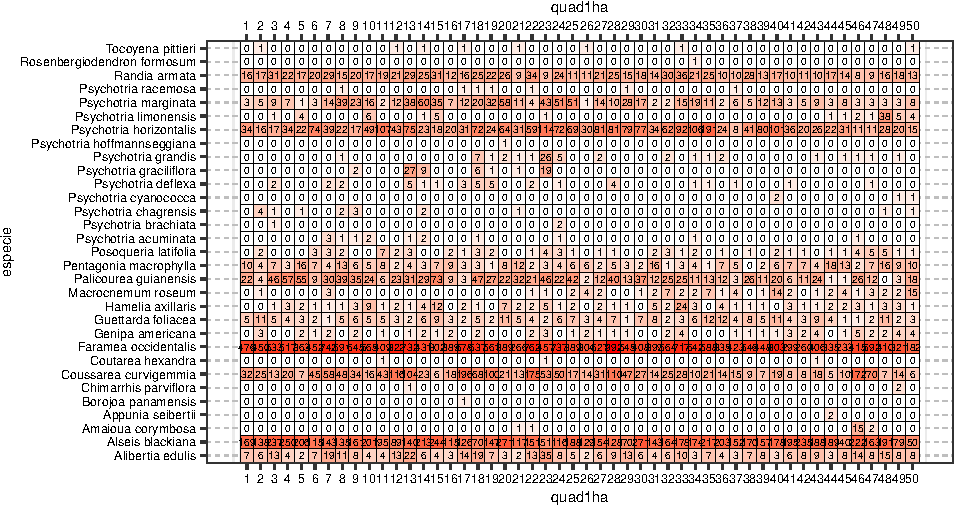
\includegraphics{manuscrito_files/figure-latex/unnamed-chunk-3-1.pdf}
Los valores para el coeficiente de Spearman presentados en el panel de
correlación de la figura \ref{fig:panel_cor_suelo_abun_riq_rubic} no
mostraron evidencia de que exista relación entre la riqueza numérica de
especies y la abundancia con las variables geomorfológicas notadas en la
matríz de variables ambientales. Sin embargo, el mismo análisis sugiere
una posible relación entre la abundancia numérica de especies y la
compososición del suelo, mostrando relación positiva con valores altos
de Aluminio y Fósforo, así como negativa, para valores altos de pH y
concentraciones de otros elementos (B, Ca, Cu, Fe, K, Mg, Mn, Zn y
Nitrógeno mineralizado).

\begin{figure}
\centering
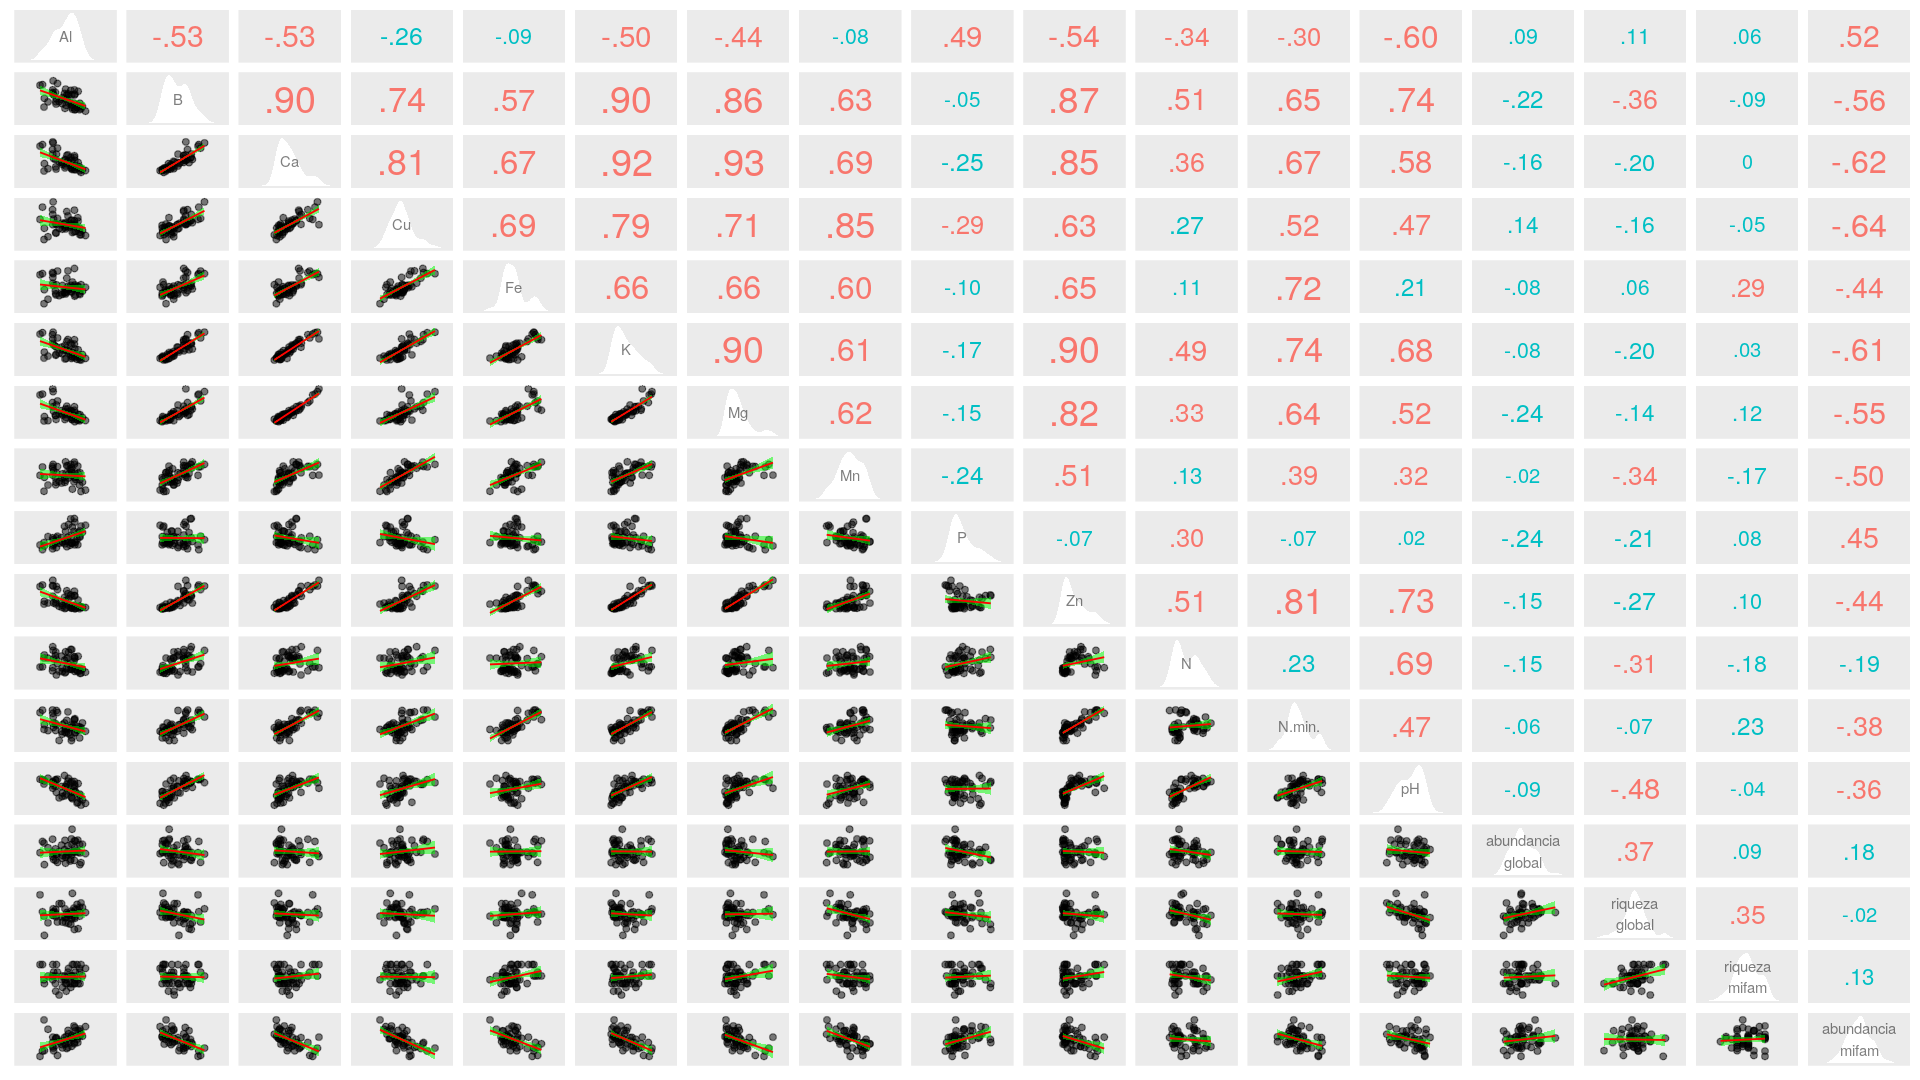
\includegraphics{panel_cor_suelo_abun_riq_rubic_spear.png}
\caption{Correlacion entre la diversidad y abundancia de rubiaceas y las
variables edafológicas \label{fig:panel_cor_suelo_abun_riq_rubic}}
\end{figure}

Las variables fósforo y cobre arrojaron valores de \emph{P} 0.0000347 y
0.0127 ``significativos'' en las pruebas T de Student respecto a los
grupos 1 y 2 formulados por complete. Otro valor de \emph{P} algo
``menos significativo'' fue 0.0808, correspondiente a la abundancia de
toda la comunidad.De manera similar, para los grupos producidos mediante
Ward, el valor \emph{P} para la variable fósforo fue de 0.000370 y
0.00726 para cobre. Otros valores para otras variables fueron: 0.0341
(Manganeso), 0.0454 (hierro), 0.0243 y 0.0331 (riqueza y abundancia
global). Las especies \emph{Alseis blackiana} y \emph{Psychotria
limonensis} fueron las especies que obtuvieron un alto valor de
confianza en los análisis de especies indicadoras del grupo 1 (grupo 2
en Ward). Para el caso del grupo 2 (1 en Ward), las especies indicadoras
fueron \emph{Faramea occidentalis}, \emph{Psychotria horizontalis} y
\emph{Coussarea curvigemmia}. Las ocurrencia de \emph{A. blackiana} y
\emph{Pentagonia macrophylla} indican su preferencia por el grupo 1
(complete). Por otra parte, en el grupo 2 (complete) siete especies
resultan de interes por su ocurrencia: la muy dominante \emph{F.
occidentalis}; \emph{Psychotria deflexa}, \emph{P. racemosa}, \emph{P.
horizontalis}, \emph{Posoqueria latifolia}, \emph{Alibertia edulis} y
\emph{Coussarea curvigemmia}. En los grupos generados mediante Ward solo
\emph{F. occidentalis}, \emph{P. horizontalis} y \emph{A. blackiana}
resultaron compatibles en el analisis de fidelidad de asociación. El
grupo 1 (2 en Ward) contiene los sitios con tendencia a presentar
valores altos de ácidez {[}\ref{fig:mapa_cuadros_ph}{]} y concentración
de aluminio. Los gráficos de barras \ref{fig:env_suelo_pca_bar_quebrd} y
\ref{fig:env_geomorf_pca_bar_quebrd} muestran los componentes
principales de la varianza en las variables de componentes del suelo y
geomorfológicas de BCI. La varianza acumulada de los PC1 y PC2 logran
explicar el 73.1\% y el 43.6\% de la varianza total respectivamente. En
estos gráficos se incluyen los valores predichos por el modelo de la
bara quebrada representado por la línea roja formando la curva.

\begin{figure}
\centering
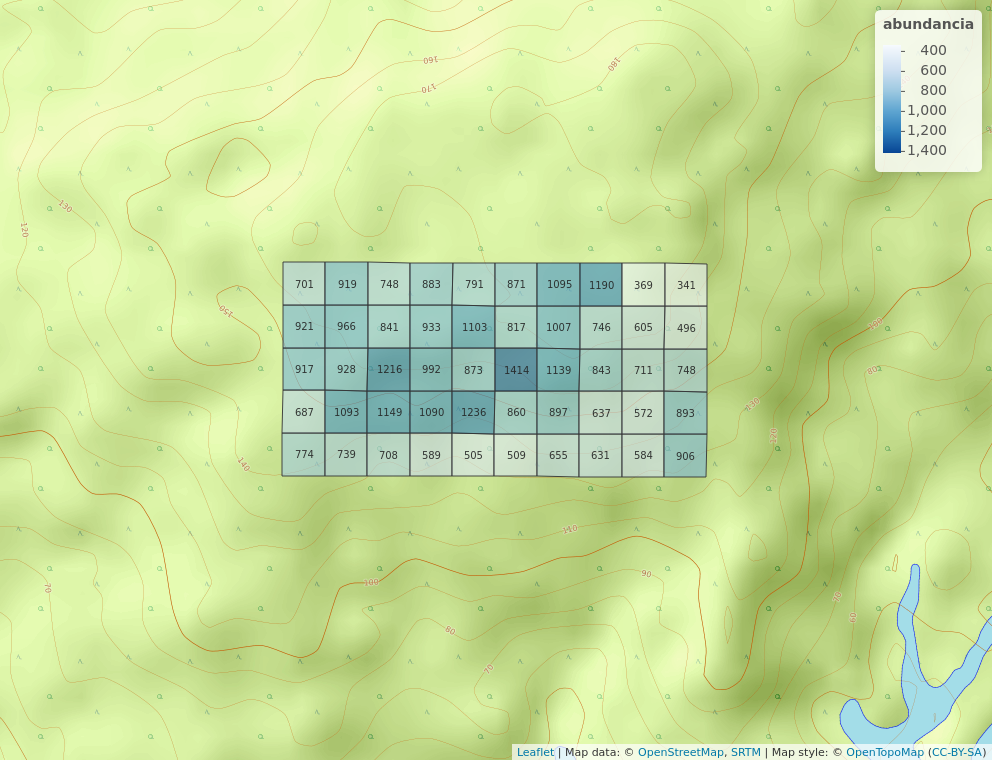
\includegraphics{mapa_cuadros_abun_rubic.png}
\caption{Abundancia de rubiaceas en BCI
\label{fig:mapa_cuadros_abun_rubic}}
\end{figure}

\begin{figure}
\centering
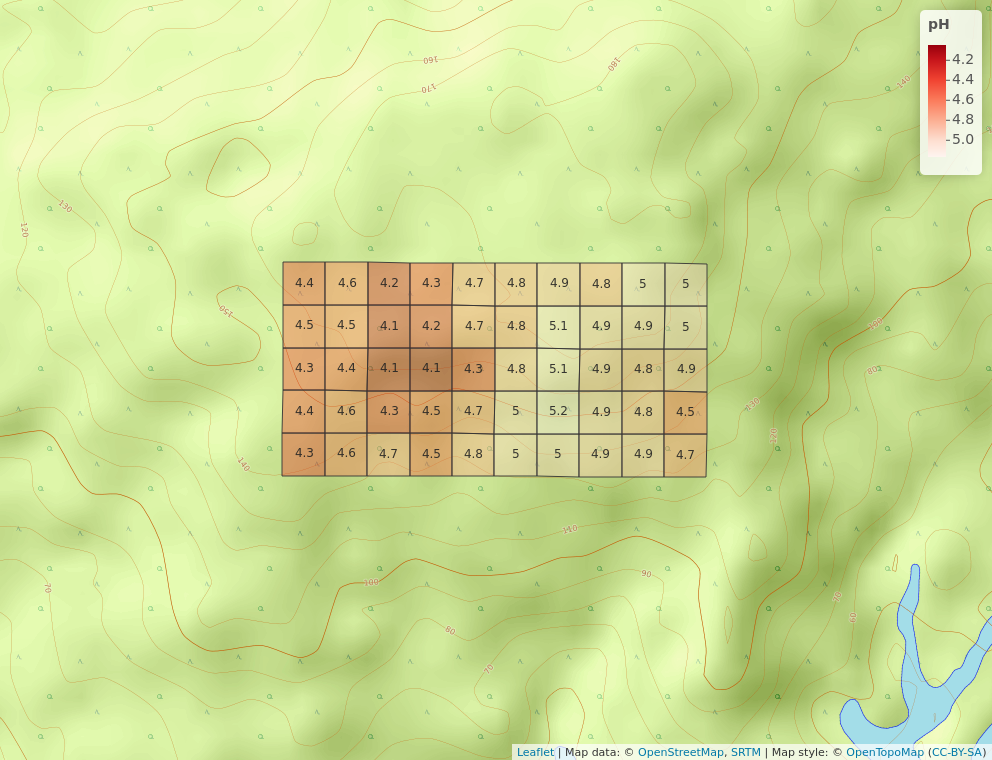
\includegraphics{mapa_cuadros_ph.png}
\caption{pH del suelo en los cuadros de 1ha \label{fig:mapa_cuadros_ph}}
\end{figure}

\begin{figure}
\centering
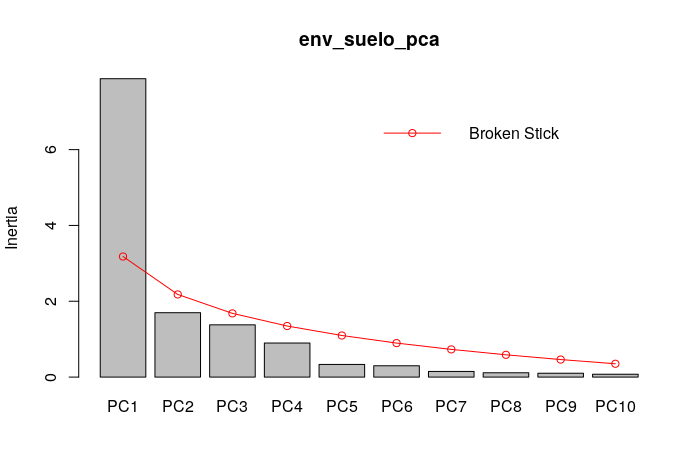
\includegraphics{env_suelo_pca_bar_quebrd.png}
\caption{Componentes príncipales de la varianza en las variables de
suelo en BCI. \label{fig:env_suelo_pca_bar_quebrd}}
\end{figure}

\begin{figure}
\centering
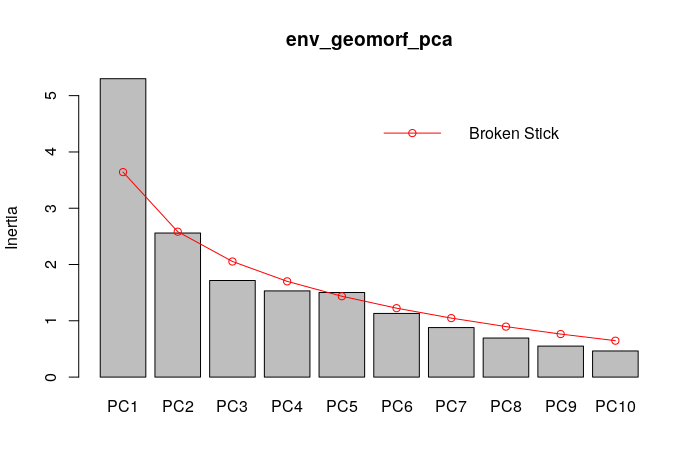
\includegraphics{env_geomorf_pca_bar_quebrd.png}
\caption{Componentes príncipales de la varianza en la geomorfología de
BCI. \label{fig:env_geomorf_pca_bar_quebrd}}
\end{figure}

\section{Discusión}\label{discusiuxf3n}

La determinación de las especies indicadoras \emph{Faramea occidentalis}
y \emph{Alseis blackiana} de los grupos uno y dos puede estár asociada a
la dominancia que presentan estas especies en la comunidad de rubiaceas.
Especialmente \emph{F. occidentalis}, cuya abundancia alcanza valores
extremos dentro de todo BCI e incluso podría estar inclinando los
resultados de estos analisis?. Las especies con preferencia por el grupo
1, evaden sistemáticamente al grupo 2, su ocurrencia se ve marcada por
algun otro factor que determina la existencia de esta diferenciacion.
Esto sucede de la misma manera para las especies con preferencia por el
grupo 2. Los análisis de agrupamiento pueden verse sesgados por la
heterogeneidad morfométrica que pueden presentar las plantas de esta
familia. Estas especies presentan diversos hábitos de crecimiento, desde
porte herbáceo y arbustivo a árboles relativamente grandes. Esto hace
que el hecho de que se incluya el criterio de dap de 10 mm en el momento
de ser censadas podría estar excluyendo especies clave en el
rompecabezas.

\section{Agradecimientos}\label{agradecimientos}

\section{Información de soporte}\label{informaciuxf3n-de-soporte}

\ldots

\section{\texorpdfstring{\emph{Script}
reproducible}{Script reproducible}}\label{script-reproducible}

\ldots

\section*{Referencias}\label{referencias}
\addcontentsline{toc}{section}{Referencias}

\hypertarget{refs}{}
\hypertarget{ref-cita_mapview}{}
Appelhans, T., Detsch, F., Reudenbach, C., \& Woellauer, S. (2019).
\emph{Mapview: Interactive viewing of spatial data in r}. Retrieved from
\url{https://CRAN.R-project.org/package=mapview}

\hypertarget{ref-borcard_legendre}{}
Borcard, D., Gillet, F., \& Legendre, P. (2018). \emph{Numerical Ecology
with R. Second Edition} (pp. 52--66).
\url{https://doi.org/10.1007/978-3-319-71404-2}

\hypertarget{ref-caceres2009associations}{}
Cáceres, M. D., \& Legendre, P. (2009). Associations between species and
groups of sites: Indices and statistical inference. \emph{Ecology},
\emph{90}(12), 3566--3574.

\hypertarget{ref-condit_et_al_2012}{}
Condit, R., Chisholm, R. A., \& Hubbell, S. P. (2012). Thirty years of
forest census at Barro Colorado and the importance of immigration in
maintaining diversity. \emph{PLOS ONE}, \emph{7}(11), 1--6.
\url{https://doi.org/10.1371/journal.pone.0049826}

\hypertarget{ref-condit_et_al_2017}{}
Condit, R., Pérez, R., Lao, S., Aguilar, S., \& Hubbell, S. P. (2017).
Demographic trends and climate over 35 years in the Barro Colorado 50 ha
plot. \emph{Forest Ecosystems}, \emph{4}(1), 17.
\url{https://doi.org/10.1186/s40663-017-0103-1}

\hypertarget{ref-article_condit}{}
Condit, R., Pitman, N., Leigh, E., Chave, J., Terborgh, J., Foster, R.,
\ldots{} Hubbell, S. (2002). Beta-diversity in tropical forest trees.
\emph{Science (New York, N.Y.)}, \emph{295}, 666--669.
\url{https://doi.org/10.1126/science.1066854}

\hypertarget{ref-davis2009global}{}
Davis, A. P., Govaerts, R., Bridson, D. M., Ruhsam, M., Moat, J., \&
Brummitt, N. A. (2009). A global assessment of distribution, diversity,
endemism, and taxonomic effort in the rubiaceae1. \emph{Annals of the
Missouri Botanical Garden}, \emph{96}(1), 68--78.

\hypertarget{ref-cita_indicspecies}{}
De Caceres, M., \& Legendre, P. (2009). Associations between species and
groups of sites: Indices and statistical inference. In \emph{Ecology}.
Retrieved from \url{http://sites.google.com/site/miqueldecaceres/}

\hypertarget{ref-dufrene_legendre}{}
Dufrene, M., \& Legendre, P. (1997). Species assemblages and indicator
species: The need for a flexible asymmetrical approach. \emph{Ecological
Monographs}, \emph{67}, 345--366. \url{https://doi.org/10.2307/2963459}

\hypertarget{ref-hubell_foster_1983}{}
Hubbell, S. P., \& Foster, R. B. (1983). Diversity of canopy trees in a
neotropical forest and implications for conservation. In T. Whitmore, A.
Chadwick, \& A. Sutton (Eds.), \emph{Tropical rain forest: Ecology and
management} (pp. 25--41). Oxford: The British Ecological Society.

\hypertarget{ref-hubell_et_all_1990}{}
Hubbell, S. P., Condit, R., Foster, R. B., Grubb, P. J., Thomas, C. D.,
Hassell, M. P., \& May, R. M. (1990). Presence and absence of density
dependence in a neotropical tree community. \emph{Philosophical
Transactions of the Royal Society of London. Series B: Biological
Sciences}, \emph{330}(1257), 269--281.
\url{https://doi.org/10.1098/rstb.1990.0198}

\hypertarget{ref-web_bci}{}
Hubbell, S., Condit, R., \& Foster, R. (2021). Forest Census Plot on
Barro Colorado Island. Retrieved March 23, 2021, from
\url{http://ctfs.si.edu/webatlas/datasets/bci/}

\hypertarget{ref-article}{}
Jansen, S., Robbrecht, E., Beeckman, H., \& Smets, E. (2000). Aluminium
accumulation in rubiaceae: An additional character for the delimitation
of the subfamily rubioideae? \emph{IAWA Journal}, \emph{21}.
\url{https://doi.org/10.1163/22941932-90000245}

\hypertarget{ref-legendre_galllagher_2001}{}
Legendre, P., \& Gallagher, E. (2001). Ecologically meaningful
transformations for ordination of species data. \emph{Oecologia},
\emph{129}, 271--280. \url{https://doi.org/10.1007/s004420100716}

\hypertarget{ref-jose_ramon_martinez_batlle_2020_4402362}{}
Martínez Batlle, J. R. (2020).
biogeografia-master/scripts-de-analisis-BCI: Long coding sessions
(Version v0.0.0.9000). \url{https://doi.org/10.5281/zenodo.4402362}

\hypertarget{ref-moreno2001manual}{}
Moreno, C. E. (2001). \emph{Manual de métodos para medir la
biodiversidad}. Universidad Veracruzana.

\hypertarget{ref-2008arXiv0803.3704N}{}
Néda, Z., Horvat, S., Toháti, H. M., Derzsi, A., \& Balogh, A. (2008). A
spatially explicit model for tropical tree diversity patterns.
\emph{arXiv E-Prints}, arXiv:0803.3704.

\hypertarget{ref-cita_vegan}{}
Oksanen, J., Blanchet, F. G., Friendly, M., Kindt, R., Legendre, P.,
McGlinn, D., \ldots{} Wagner, H. (2019). \emph{Vegan: Community ecology
package}. Retrieved from \url{https://CRAN.R-project.org/package=vegan}

\hypertarget{ref-cita_sf}{}
Pebesma, E. (2018). Simple Features for R: Standardized Support for
Spatial Vector Data. \emph{The R Journal}, \emph{10}(1), 439--446.
\url{https://doi.org/10.32614/RJ-2018-009}

\hypertarget{ref-cita_r}{}
R Core Team. (2020). \emph{R: A language and environment for statistical
computing}. Retrieved from \url{https://www.R-project.org/}

\hypertarget{ref-TORRESLEITE2019151487}{}
Torres-Leite, F., Cavatte, P. C., Garbin, M. L., Hollunder, R. K.,
Ferreira-Santos, K., Capetine, T. B., \ldots{} Carrijo, T. T. (2019).
Surviving in the shadows: Light responses of co-occurring rubiaceae
species within a tropical forest understory. \emph{Flora}, \emph{261},
151487.
\url{https://doi.org/https://doi.org/10.1016/j.flora.2019.151487}

\hypertarget{ref-Volkov_2003}{}
Volkov, I., Banavar, J. R., Hubbell, S. P., \& Maritan, A. (2003).
Neutral theory and relative species abundance in ecology. \emph{Nature},
\emph{424}(6952), 1035--1037. \url{https://doi.org/10.1038/nature01883}

\hypertarget{ref-cita_tidyverse}{}
Wickham, H. (2017). \emph{Tidyverse: Easily install and load the
'tidyverse'}. Retrieved from
\url{https://CRAN.R-project.org/package=tidyverse}




\newpage
\singlespacing 
\end{document}
